In this section, we divide the problem into subproblems, and analyse them separately.

We can divide the requirements into the two following subproblems.
\begin{itemize}
 \item \emph{The editor.} We need to show the conveyor belt system, and enable the user to edit it by adding new conveyor belts and removing them. This includes a GUI for the user to for example choose blocks.
 \item \emph{The simulator.} We need to simulate and show movement of luggage over the conveyor belts.
\end{itemize}
We can subdivide the editor again in several parts.
\begin{itemize}
 \item \emph{Viewing conveyor belts.} We need to show the conveyor belt system to the user in 3D.
 \item \emph{The interface.} We need to have an interface with which the user can choose different kinds of blocks, rotate them, and so on.
 \item \emph{Placing blocks.} Finally, the user needs to have a way to indicate where blocks should be placed or removed; therefore, we need to be able to convert 2D mouse clicks to the corresponding 3D location.
\end{itemize}

\subsection{Viewing}
\label{subsec:analysis-viewing}
For viewing the conveyor belt system, it is of course important that the user is able to see the properties of every conveyor belt clearly. That is, the following three properties should be visible:
\begin{itemize}
  \item the \textit{shape} (is it horizontal, ascending\,/\,descending or a bend);
  \item the \textit{orientation} (is the conveyor belt oriented in the $x$- or the $y$-direction);
  \item the \textit{direction} (towards which of the two possible directions does it move).
\end{itemize}
The first two properties do not need a lot of realism: only a rough approximation of the shape will suffice for that. However, for the user to be able to see the direction, just the drawn shape will not be enough.

In the building mode, we can simply draw arrows on top of the conveyor belts that indicate the direction. During the simulation however, we think that looks very bad. Instead, we want the conveyor belts to look like they really move. To do this in an easy way, we can use a texture on the surface of the conveyor belt, and animate its texture coordinates.

We can use a texture of a small part of the conveyor belt, and repeat it in the length direction of the belt. A requirement is then that the texture does not get deformed, that is, the texture coordinates should be such that every repetition of the texture has (about) the same size. This is especially important since we are going to animate the texture, meaning that deformations in the texture would become visible as stretching or shortening of parts of the conveyor belt.

\subsubsection{What is the problem?}
\label{subsubsec:texture-coord-problem}
Let us look at what the problem is in detail, before giving our solution in Section~\ref{subsubsec:texture-coord-calculate}. Recall that we want to indicate to the user that the conveyor belts are moving and that we want to do so by texturing the belts. This means that we map a 2D texture to the 3D surface of a conveyor belt. This is straightforward: if we only consider the top of each conveyor belt (the bottom is symmetric), then this is a surface in 3D that has a left and a right side. This is true because any conveyor belt block in our program has a fairly restricted shape. We can now map the left side of our texture to the left side of this 3D surface and similarly map the right side of our texture to the right side of the 3D surface and we are done. So, no problem? Not if we only consider one block. However, we have more requirements:
\begin{itemize}
  \item As said before, they should not deform the texture (or only a little bit). Said differently, there is some $r$ such that for every point $p$ on the belt,
  \[
    l(p) \approx r \cdot t(p),
  \]
  where $l(p)$ means the length of the belt until point $p$ and $t(p)$ denotes the texture coordinate at point $p$.
  \item Furthermore, we want the blocks to be tileable. As described in section~\ref{subsubsec:drawing-adjacent}, we want to draw adjacent blocks as one large conveyor belt. Therefore, we require that $t(p) \in \mathbb{N}$ for points $p$ that connect to other belts.
  \item Finally, we do not want the texture coordinates to become very high, since that means that the texture will be repeated many times on the conveyor belt, which may become noticeable.
\end{itemize}
The problem is mostly in the second requirement, that the texture must be tileable. This requirement basically states that the texture maps for different shapes of conveyor blocks have a relation to each other: if two shapes are drawn next to each other, then the texture maps must form a whole, they must connect seamlessly with each other. Consider two flat conveyor belts that are drawn next to each other (the top situation in Figure~\ref{fig:blocks-adjacent}) and for the sake of simplicity, only consider the top of these belts. The surfaces of both conveyor belts now consist of a quarter of a circle arc and some straight line, when looking from the side. This directly implies that the length of that surface is not a natural number: the length of the circumference of a circle is $2 \cdot \pi \cdot r$, where $r$ is the radius of the circle and $\pi \not\in \mathbb{N}$. We can pick $r = \frac{k}{2 \cdot \pi}$ for some $k \in \mathbb{N}$, however that implies that the length of the straight surface after the arc is not a natural number anymore. If the length of one conveyor belt block is $l$, then the length of the straight surface is $l - r$, which cannot be a natural number if $l \in \mathbb{N}$ and $r \not\in \mathbb{N}$.

\subsubsection{Calculating texture coordinates}
\label{subsubsec:texture-coord-calculate}
For calculating the texture coordinates, we use the following strategy: we use fixed values for every point at the conveyor belt, and then we animate those linearly. Assuming that the fixed values indeed do not deform the texture too much, the animated texture will also not be deformed in this way.

The problem left now is determining the fixed values while respecting the requirements described in Section~\ref{subsubsec:texture-coord-problem}. We tried to find an exact solution, but this turns out to be hard, especially since the requirements are quite vague. Finally, we came up with an approximate solution manually, that is shown in Figure~\ref{fig:sketch-texturing}. Note that it basically uses that $\pi \approx 3$. We used similar approximate texture mappings for other conveyor shapes. For example, for the \eo{ascending}{descending} conveyor belts, we used that the length of the side, which is $\sqrt{1^2 + (1/4)^2} = 1.0625 \approx 1$. We found that this solution works well in practice.
\begin{figure}
  \begin{center}
    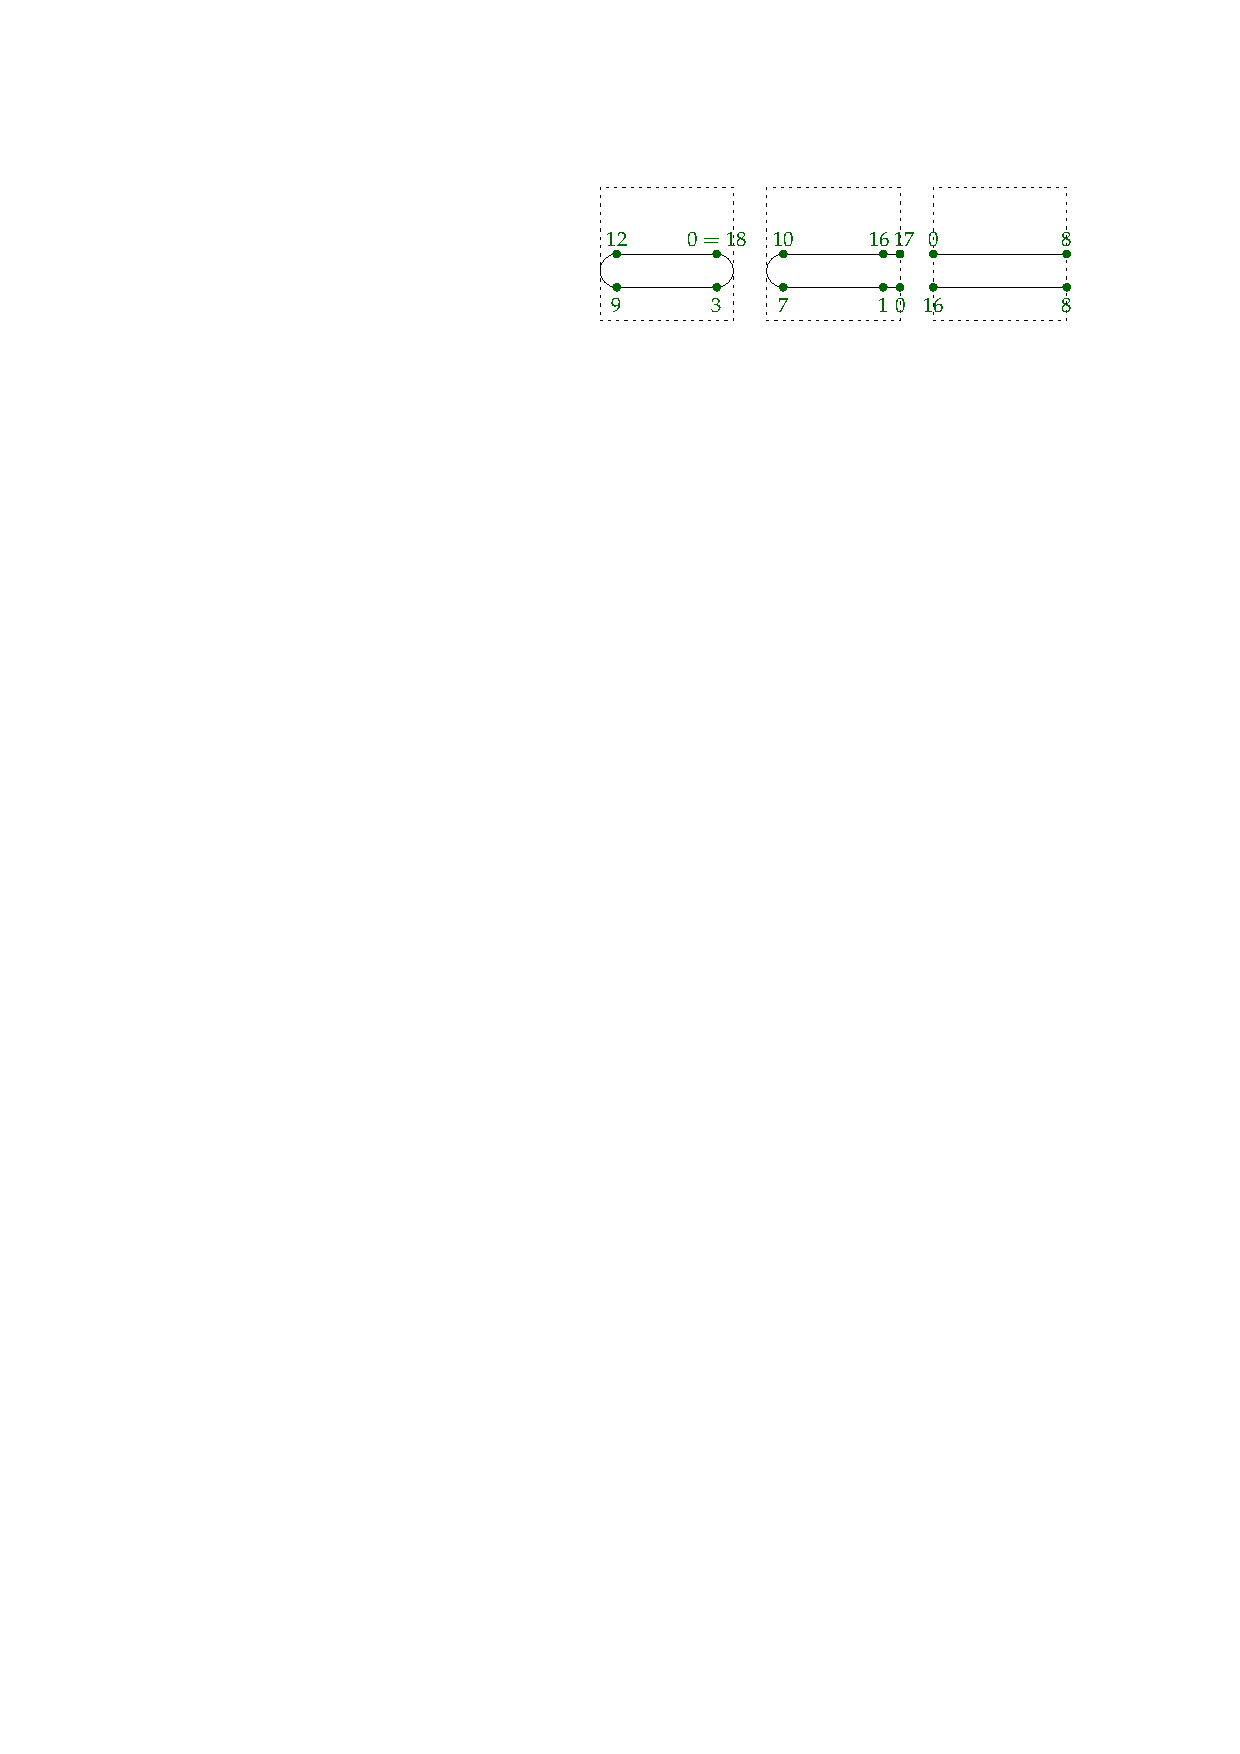
\includegraphics{sketch-texturing}
    \caption{Texture coordinates for the horizontal conveyor belt.}
    \label{fig:sketch-texturing}
  \end{center}
\end{figure}

\subsubsection{Drawing adjacent conveyor belts}
\label{subsubsec:drawing-adjacent}
When two conveyor belts are adjacent to each other, they should be drawn as one large belt. (This makes sense, since probably in real systems also one long belt would be used instead of many short ones.) See Figure~\ref{fig:blocks-adjacent} for a sketch.
\begin{figure}
  \begin{center}
    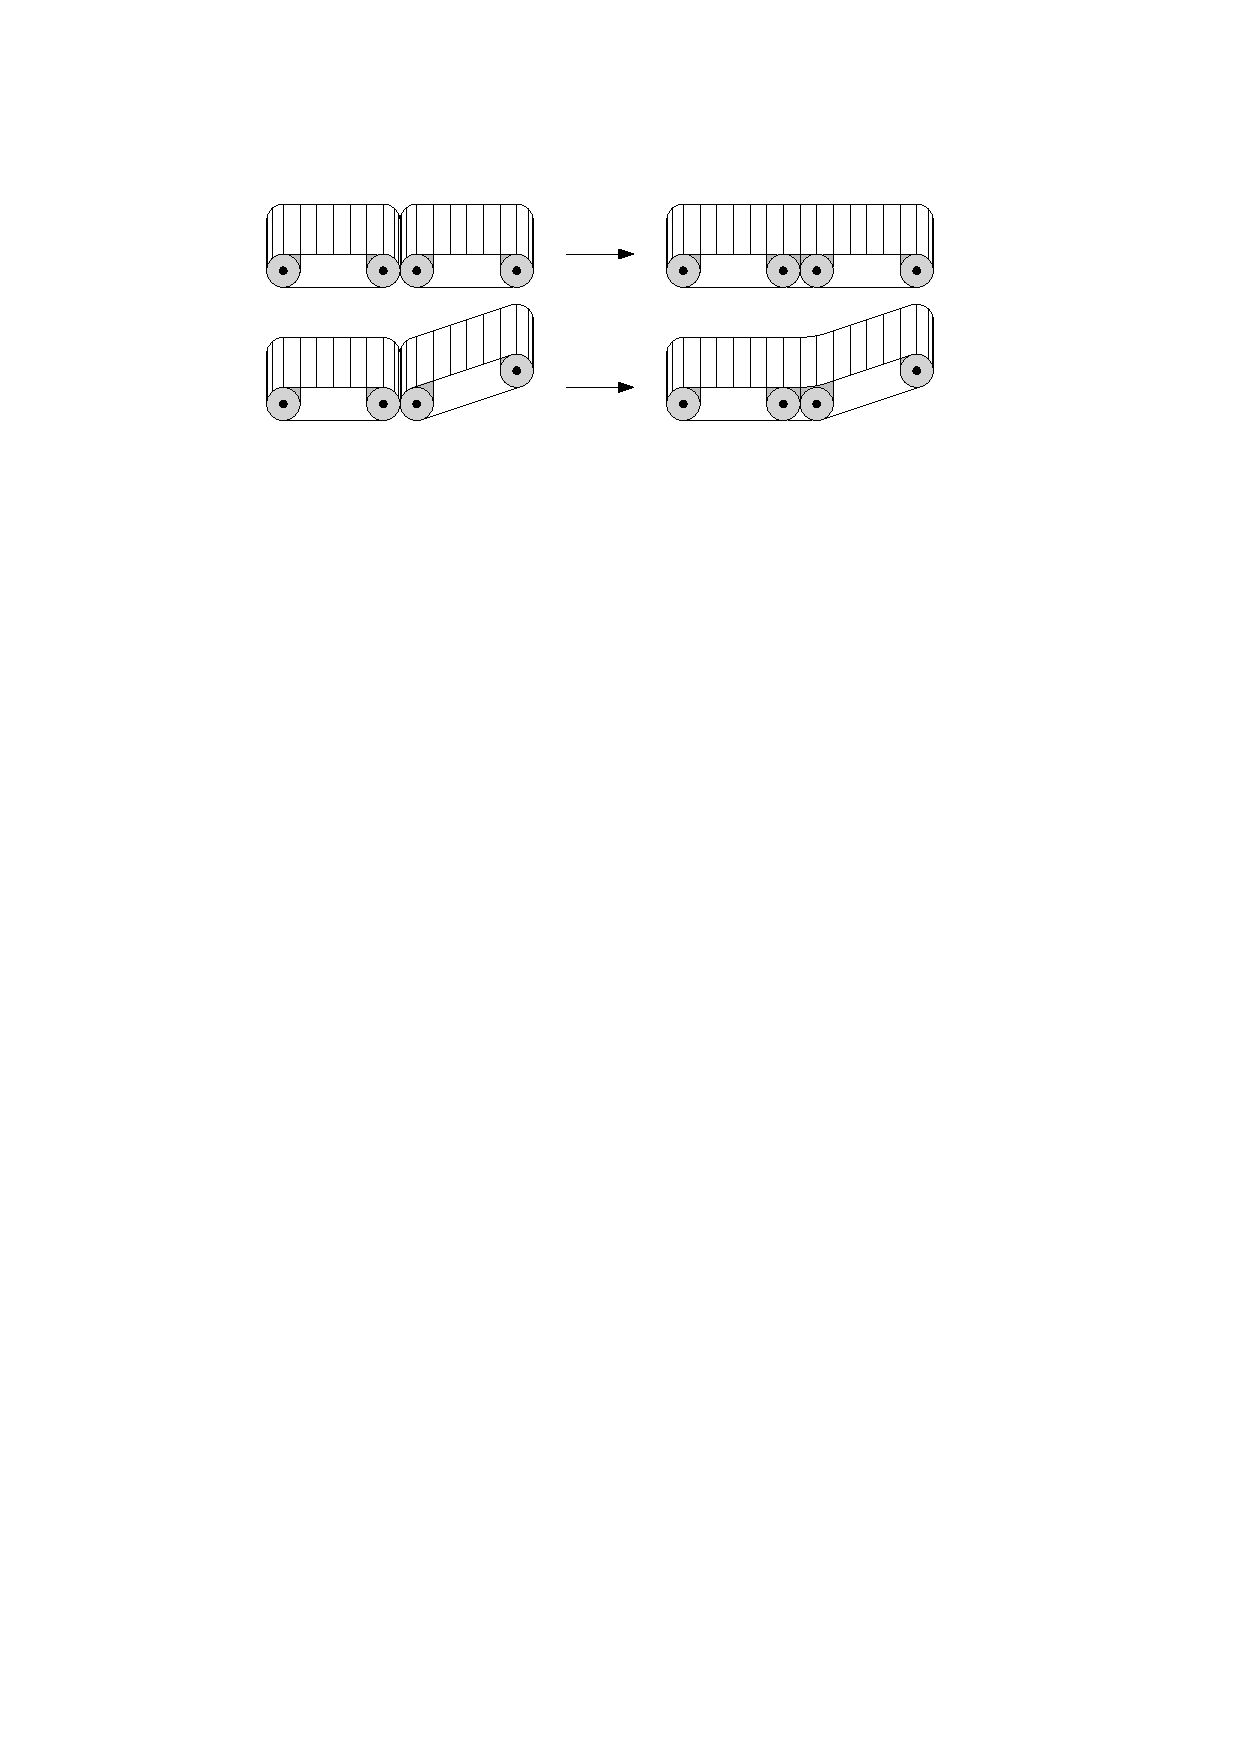
\includegraphics{blocks-adjacent}
    \caption{Adjacent blocks should be drawn together.}
    \label{fig:blocks-adjacent}
  \end{center}
\end{figure}

This is not only a feature for realism, but it also is an additional clue for the user to view the conveyor belt system easier. Namely, when one large belt is shown, the user can be sure that the belts are correctly adjacent to each other and that they all have the same direction.


\subsection{Interface}
\label{subsec:analysis-interface}
We discussed in Section~\ref{subsubsec:design-goals-editor} what we expect from the interface of the program. Since we plan to implement our tool in Java, using a thin wrapper\footnote{LWJGL to be precise, see \url{http://lwjgl.org/}.} around OpenGL, we will have to use some kind of GUI toolkit, or write our own. We did a quick search and did not find any useful toolkits, so we will write our own (basic) GUI toolkit. This toolkit should be able to render components in OpenGL, using the 2D OpenGL capabilities to render a GUI on top of the 3D scene. It should furthermore be easily extendable, flexible in the sense that placements of menu bars should be configurable for example and finally it must be capable of handling input events quickly and without complex API. Since we want everything to look good, the toolkit should support buttons (in menu bars) with icons and a configurable font. Preferably, the toolkit also supports animations. For example, when a button is hovered, its background colour may change. This change might be animated, simply because it looks good.

If we add tooltips to our menu items and buttons, the toolkit must be of course able to render those. Preferably, tooltips are shown and hidden with a fading animation, but this is not a hard requirement. In case the toolkit does support animations at all, it would however be good if it does so in a as-generic-as-possible way, so that the functionality can be used for different purposes (hover animations, tooltip animations, \ldots).

\subsubsection{Switching between program modes}
\label{subsubsec:switch-program-modes}
There are multiple modes in which the program can be. In Section~\ref{sec:introduction} the building mode was discussed shortly. There are two other modes in which the program can be. We list those modes below. The interface should provide a way to switch between those modes in an intuitve way, for example via a button or menu item. The interface may also provide shortcuts to switch.
\begin{longtabu} to \linewidth {lX<{\strut}}
  \toprule
  \textit{Program mode} & \textit{Description} \\
  \midrule
  \endhead
  \bottomrule
  \endfoot
  Normal mode & The program starts up in this mode. The user can do the following: switching to another mode, control the camera freely to view the scene from any angle he/she likes, saving his/her conveyor belt system, loading a system or changing settings.  \\
  Building mode & In building mode, the user can place new conveyor blocks in the scene. See Section~\ref{subsubsec:interface-placing-blocks} for details. It should also be possible to go to the simulation mode to test the conveyor belt system. \\
  Simulation mode & In the simulation mode, luggage is introduced to the conveyor belt system. The user can control the camera freely to see how his/her system behaves. It is possibly to stop the simulation, returning to the building mode. It may be possible to pause/continue the simulation. \\
\end{longtabu}

\subsubsection{Interface for placing blocks}
\label{subsubsec:interface-placing-blocks}
In the building mode (see Section~\ref{subsubsec:switch-program-modes}) the user should be presented with an intuitive interface to place new blocks quickly. It should be possible to click an existing block or place a new block by clicking the floor and then optionally dragging the block upwards to the desired height. In both cases, after that a special interface should be shown which the user can use to build a block from the lastly placed (or selected) block. The camera should look in the direction in which the user is building and this direction should be indicated by an arrow. It should be possible to select the next block that will be placed or go back to a free camera mode to place a new block or select another one. The special interface that is shown when building blocks should present the user with all different types of block, to change which block is being built next. It should also make it possible for the user to delete the lastly built (or selected) block. Finally, an option to change the direction of the next block should be presented (rotate left and rotate right). Of course, the direction in which is being built must change automatically in case a curved conveyor belt is being built.

\subsection{Placing}
\label{subsec:analysis-placing}
Test.

\subsection{Simulation}
\label{subsec:analysis-simulation}
We saw in Section~\ref{subsubsec:design-goals-simulator} that we have quite a number of constraints on the simulator. We realised that we would need to use a physics library, which is exactly what we will do. Hence, the problem of simulating the movement of pieces of luggage over the conveyor belts is most likely a matter of understanding the API of the library we are going to use and then using it correctly. We may also have to synchronise the speed of the conveyor belts in the library with the animation speed of the conveyor belts in OpenGL.